\documentclass[../../../../main.tex]{subfiles}

\begin{document}

\section*{第1問}

\begin{proof}[解]
\textbf{$1^\circ$ $(a,b)=(0,0)$の時}

題意は成立。

\textbf{$2^\circ$ $a=0,\ b\ne0$の時}

$a^2x^2+b^2y^2\le1$をみたす$(x,y)$は，$x$：任意，$|y|\le1/|b|$であり，$1\le b$であれば良い。

\textbf{$3^\circ$ $a\ne0,\ b=0$}

$2^\circ$と同様に$1\le a$であれば良い。

以下，$ab\ne0$のもとで考える。この時，$xy$平面上で$a^2x^2+b^2y^2\le1$のグラフ上の点が$a(x-1)+b(y-1)\le0$をみたすような$(a,b)$の範囲をもとめれば良い。$(x,y)=\left(\dfrac{r}{a}C,\dfrac{r}{b}S\right)$（$C=\cos\theta,\ S=\sin\theta,\ 0\le\theta<2\pi,\ 0\le r\le1$）とおける。これに代入して
\[
rC-a+rS-b\le0
\]
\[
r\sqrt2\sin\left(\theta+\frac{\pi}{4}\right)\le a+b
\]
が任意の$\theta,r$で成立すれば良く，その条件は
\[
a+b\ge\sqrt2
\]
以上まとめて，
\[
a=b=0 \ \text{or}\ (ab\ne0\wedge a+b\ge\sqrt2)\ \text{or}\ (a=0\wedge b\ge1)\ \text{or}\ (b=0\wedge a\ge1)
\]
図示して下図斜線部（境界，$\bullet$を含む）。

\begin{center}
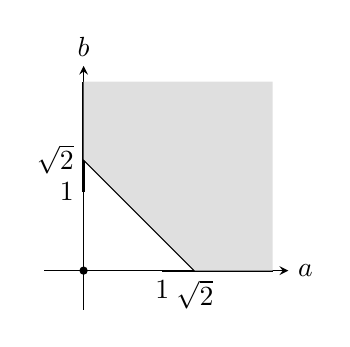
\begin{tikzpicture}[scale=1.0, >=stealth]
  \draw[->] (-0.5,0) -- (2.6,0) node[right] {$a$};
  \draw[->] (0,-0.5) -- (0,2.6) node[above] {$b$};
  \draw[thick] (1.414,0) -- (0,1.414);
  \draw[thick] (1,0) -- (2.4,0);
  \draw[thick] (0,1) -- (0,2.4);
  \fill[gray!25] (1.414,0) -- (0,1.414) -- (0,2.4) -- (2.4,2.4) -- (2.4,0) -- cycle;
  \fill (0,0) circle (1.5pt);
  \node[below] at (1,0) {$1$};
  \node[below] at (1.414,0) {$\sqrt2$};
  \node[left] at (0,1) {$1$};
  \node[left] at (0,1.414) {$\sqrt2$};
\end{tikzpicture}
\end{center}
\end{proof}

\bigskip
\noindent\textbf{[別解]}

\begin{proof}[別解]
同様に$a\ne0,b\ne0$で考える。$X=ax,\ Y=by$とおく。$x^2+y^2\le1$をみたす全ての$X,Y$が$X+Y\le a+b$をみたせば良く，
\[
a+b\ge\sqrt2
\]
である。
\end{proof}

\newpage

\section*{第2問}

\begin{proof}[解]
$y=f(x)=\dfrac{1}{a+x}\ (a\ge0)$のグラフは下図で，斜線部は
\[
S_n=\sum_{k=n}^{2n}\frac{1}{a+k}
\]
の面積である。面積比較して
\[
\int_n^{2n}f(x)dx+\frac{1}{a+2n}<S_n<\int_n^{2n}f(x)dx+\frac{1}{a+n} \quad\cdots\text{①}
\]
\[
\int_n^{2n}f(x)dx=\left[\log(x+a)\right]_n^{2n}=\log\frac{2n+a}{n+a}=\log2+\log\frac{1+a/2n}{1+a/n}
\]
だから，①の最左右辺は共に$\log2$に収束するので，はさみうちの定理から
\[
S_n\longrightarrow\log2 \quad\cdots(1)
\]
これは$a$によらない。$\cdots(2)$
\end{proof}

\newpage

\section*{第3問}

\begin{proof}[解]
\textbf{(1)}
\[
\frac1x+\frac1y=\frac12
\]
\[
xy-2x-2y=0 \quad\therefore\ (x-2)(y-2)=4
\]
対称性から$x\le y$とすると，$x,y\in\mathbb{N}$から$x-2\ge-1,\ y-2\ge-1$。$(x-2)(y-2)=4>0$から，$x-2,y-2$は同符号で，共に負なら積は高々1だから，共に正で$x-2,y-2\in\mathbb{N}$。だから
\[
(x-2,y-2)=(1,4),(2,2) \quad\therefore\ (x,y)=(3,6),(4,4)
\]
$x\le y$の場合もかんがえて
\[
(x,y)=(3,6),(6,3),(4,4)
\]

\textbf{(2)} まず$x_1\ge x_2\ge\cdots\ge x_n$とする。$n=1$で明らかで，以下$n=i$での成立を仮定し，$n=i+1$での成立を示す（$i\in\mathbb{N}$）。
\[
r=\frac1{x_1}+\cdots+\frac1{x_{i+1}}\le\frac{i+1}{x_{i+1}}
\]
\[
\therefore\ x_{i+1}\le\frac{i+1}{r}
\]
これをみたす最大の自然数$N$とし，$x_{i+1}$の値で場合分けして$(x_1,x_2,\cdots,x_i,x_{i+1})$の組をかぞえれば良く，
\[
\sum_{\ell=1}^Na_i\left(r-\frac1\ell\right)
\]
とかける。ここで$a_i(r)$は$n=i$の時の$\sum\dfrac1{x_k}=r$をみたす$(x_1,\cdots,x_i)$の組の数であり，仮定から$a_i(r-1/\ell)$は有限。したがって$n=i+1$でも成立。

以上から$x_1\ge x_2\ge\cdots\ge x_n$では有限個だから，この条件をはずしても高々（有限）$\times n!$通りで，有限である。

（＊一応，条件が$r\le x_{i+1}\le\cdots\le x_1$となっているので）
\end{proof}

\newpage

\section*{第4問}

\begin{proof}[解]
\textbf{(1)} 右のように各点をおく。正弦定理から
\[
\frac{AB}{\sin\beta}=\frac{AC}{\sin\alpha}=\frac{\ell}{\sin(\alpha+\beta)} \quad\cdots\text{①}
\]
\[
S=\frac12AB\cdot AC\cdot\sin(\alpha+\beta)
\]
\[
=\frac12\cdot\frac{\ell\sin\beta}{\sin(\alpha+\beta)}\cdot\frac{\ell\sin\alpha}{\sin(\alpha+\beta)}\cdot\sin(\alpha+\beta) \quad(\because①)
\]
\[
=\frac{\ell^2}{2}\cdot\frac{\sin\alpha\sin\beta}{\sin(\alpha+\beta)}
\]
\[
=\frac{\ell^2}{4}\cdot\frac{\cos(\alpha-\beta)-\cos(\alpha+\beta)}{\sin(\alpha+\beta)}
\]

\textbf{(2)} 各辺の長さが1,2,$\sqrt3$の三角形は，$1^2+(\sqrt3)^2=2^2$から，長さ2の辺を斜辺とする直角三角形で，3つの角は$\pi/6,\pi/3,\pi/2$である。右のようにおく（$0<x<1,\ 0\le\theta\le\pi/2$）。$\triangle CDF$，$\triangle BDE$に正弦定理を用いて
\[
BD=\frac{x}{\sin\frac\pi3}\sin\theta=\frac23\sqrt3\cdot x\sin\theta
\]
\[
CD=x\cos\theta
\]
$BD+CD=1$から
\[
\left(\frac23\sqrt3\sin\theta+\cos\theta\right)x=1 \quad\cdots\text{①}
\]
以下$S=\sin\theta,\ C=\cos\theta$と書く。$\triangle DEF$の面積を$T$とおくと，
\[
T=\frac{\sqrt3}{4}x^2
\]
であり，①と$0\le x\le1$から
\[
1\le\frac23\sqrt3\cdot S+C=\sqrt{\frac73}\sin(\theta+\alpha)\le\sqrt{\frac73} \quad(\because0\le\theta\le\pi/2)
\]
（ただし，$\alpha$は$\sin\alpha=\sqrt{3/7},\ \cos\alpha=2/\sqrt7$をみたす角）である。この範囲で①とあわせて，
\[
\sqrt{\frac37}\le x\le1
\]
だから，$T$の表す形から，$T$は$x=\sqrt{3/7}$で最小値をとる。
\[
\min T=\frac{\sqrt3}{4}\cdot\frac37=\frac{3\sqrt3}{28}
\]
\end{proof}

\end{document}
